\section{Introduction}
A long lasting controversy persists in psycholinguistic research regarding the involvement of the motor system in speech perception. The motor theory of speech perception describes phoneme perception in terms of the articulatory gestures that generate it. According to this theory, the objects of speech perception are the intended phonetic gestures of the speaker, such as, ‘lip rounding’, or ‘jaw raising’ \citep{liberman1967perception, liberman1985motor}. For example, [m] consists of a labial stop gesture combined with a velum-lowering gesture. On the other hand, auditory theories argue that phonetic processing depends directly on properties of the auditory system \citep{jakobson1951preliminaries, stevens1972quantal, stevens1989quantal, stevens2002toward}. According to this view, listeners identify spectrotemporal patterns in the phoneme waveforms and match them to stored acoustic representations. For example, vowels are characterized by a roughly bimodal spectra and sibilant fricatives by high-frequency energy.


The fundamental motivation of the motor theory arose from an early observation that phoneme percepts are invariant across different contexts \citep{cooper1952some, liberman1967perception}. In the case of coarticulation, several gestures overlap in time, which may cause the acoustic waveform of the same intended gesture to be significantly different than when it is pronounced in isolation. Therefore, a particular gesture can be represented by different acoustic waveforms in different phonetic contexts. Additional variation exists in the acoustic signal due to inter-speaker variability.  This considerable variability led the supporters of the motor theory to propose that the objects of speech perception are not to be found in acoustics.

Phoneme perception has been the focus of many neuroimaging studies \citep{liebenthal2005neural, dehaene2005neural, mottonen2006perceiving, desai2008left, liebenthal2010specialization,  formisano2008saying, binder2000human, Dewitt2012}. One common method in these studies uses sophisticated baselines to speech, such as rotated speech, to elicit activation in regions that are selective to speech, but not to nonphonemic contrasts.  The results describe a complex picture of hierarchically-organized phoneme processing in the temporal lobe, from primary auditory and early posterior auditory areas to higher-level processing in the anterior, ventral STG and STS. 

Invasive electrophysiological recordings in humans provide a precious glimpse into the neural representations of linguistic entities, such as the objects of speech perception, with high temporal resolution and spatial localization compared to non-invasive recording techniques. Several recent studies, using Electrocorticography (ECoG) grids, have contributed to our understanding of neural encoding in higher-level auditory cortex, and shed new light on the long-lasting debate in speech perception. \citet{pasley2012reconstructing} showed that speech waveforms can be reconstructed from neural activity in the lateral STG, suggesting that encoded information in this region is mainly acoustic. More recently, \citet{Mesgarani2014} have characterized the functional organization of phonemes in the peri-Sylvian speech cortex. The study provides a detailed examination of neural representations of phonemes in the STG of human subjects, during listening to natural speech. Examining the functional organization in this region, they found that phoneme representations cluster according to acoustic features, in an hierarchical manner. Remarkably, the dominant organizing acoustic features are the same distinctive features defined by linguists half a century ago \citep{ChomskyHalle1968}. Moreover, an order was found among the features: manner-of-articulation features produce a neural invariance that is more prominent than that related to place-of-articulation (more recently, a similar order was found also using EEG recordings \citep{khalighinejad2017dynamic}). This order is consistent with an early observations from language acquisition, according to which manner-of-articulation distinctions are acquired early during childhood, compared to the place-of-articulation ones \citep{jakobson1968child, grodzinsky2014neural}. Taken together, these findings support the auditory view of speech perception rather than gestural theories. Other ECoG studies have further examined the functional organization of phonemes outside the STG, and tested its dependency on the experimental task (listening vs. production). Results show that the organization can significantly differ across brain regions and tasks: \citet{bouchard2013functional} showed that the functional organization of phonemes in the vSMC during production is dominated by place-of-articulation features (e.g., labial, alveolar, velar and glottal), in contrast to manner-of-articulation features in the STG during listening. More recently, the functional organization in the same region was found to differ also across tasks. Whereas during phoneme production, the dominant organizing feature of neural activity in the vSMC is place-of-articulation, during listening, the organization in the same region was found to be dominated by manner features, similarly to the STG \citep{cheung2016auditory}.

ECoG studies have greatly enriched our understanding of the neural basis of speech perception.  However, the electrical activity recorded in ECoG grids reflects average responses of large neuronal populations, as non-invasive methods, and is therefore limited in providing insights into activity patterns of single cells. Describing and construing single-cells activity is indispensable for a complete theory of the neural basis of speech perception, and cognitive processes in general. Single-unit recording was pioneered at the mid of the previous century, and was later developed to obtain multiple single-unit recordings from deep brain structures in humans \citep{fried1999cerebral} (for a review, \citealp{engel2005invasive, mukamel2012human, cash2015emergence}). It provides unique spatiotemporal resolution and valuable information about processes that are unique to humans, such as language \citep{heit1988neural, ojemann1988neuronal, tankus2012structured, ossmy2015decoding}.

Consistent with findings from ECoG and EEG studies, single-cell studies on phonetic processing revealed a multidimensional neural representation of phonemes by demonstrating that STG neurons are tuned to subsets of phonemes and have a sparse coding scheme \citep{creutzfeldt1989neuronal, chan2013speech}. However, the functional organization of phonemes at the cellular level is still poorly understood. Specifically, whether single STG neurons encode phonemes in an hierarchical way, as was revealed by analyzing gamma activity in ECoG studies, with larger invariance to manner- compared to place-of-articulation features.

In this study, we recorded spiking activity from the superior temporal gyrus of six neurosurgical patients while they listened to simple speech stimuli in the form of consonant-vowel (CV) pairs, generated by three speakers. We characterized STG single-cell responses to the stimuli, and examined the functional organization of phonemes as revealed by single-cells activity. In particular, we addressed the question about the dominating organizing dimension, by quantifying manner- and place-of-articulation invariances, using probabilistic modelling.

The study also examines the relation between the functional organization of phonemes as revealed by single-cells activity, and the cognitive one as estimated from behavioral data. We collected phoneme-confusion rates from normal subject, using the same set of stimuli as in the experiment with neurosurgical patients. We then quantified the extent to which the cognitive and neural functional organizations correspond. 

\section{Materials and methods}
\subsection{Patients and electrophysiological recording}
Data was collected from six patients with pharmacologically intractable epilepsy, implanted with intracranial depth electrodes to identify seizure focus for potential surgical treatment \citep{mukamel2012human}. Electrode location was based solely on clinical criteria. Each electrode terminated in a set of nine 40-$\mu$m platinum–iridium microwires \citep{fried1999cerebral} — eight active recording wires, referenced to the ninth. Signals from these microwires were recorded at 40 kHz using a 64-channel acquisition system. Before surgery each patient underwent placement of a stereotactic headframe, and then a detailed MR image was obtained using a spoiled-gradient sequence, followed by cerebral angiography. Both anatomical and angiography images were transmitted to a workstation in the operating room, and surgical planning was then performed, with selection of appropriate temporal and extra-temporal targets and appropriate trajectories based on clinical criteria. To verify electrode position, CT scans following electrode implantation were co-registered to the preoperative MRI using Vitrea® (Vital Images Inc.). The patients provided written informed consent to participate in the experiments. The study was approved by and conformed to the guidelines of the Medical Institutional Review Board at UCLA and Ichilov.

\subsection{Stimuli and behavioral task}
Stimuli were constructed of either consonant-vowel (CV) pairs, or vowels /aeiou/ presented in isolation. The consonants in the CV syllables were according to the list in Table A.1, and the vowel was set to /a/ in order to reduce effects on the preceding consonant. To increase data size, we collected recordings from both Hebrew- and English-speaking patients. We therefore focused on a phoneme set that is approximately shared for both languages. Patients  were presented with 12 repetitions from each CV pair or vowel, 4 from each speaker, in a random order (ISI = 1 second). The patients were instructed to listen carefully to the syllables.

All stimuli were recorded in an anechoic chamber with a RØDE NT2-A microphone and a Metric Halo MIO2882 audio interface, at a sampling rate of 44.1kHz. Stimuli were generated by two male and one female speakers. The total number of stimuli was 63 (21 phonemes * 3 speakers). Length and pitch (by semi-tone intervals) were compared across recorded tokens to choose the most highly comparable stimulus-types. This was done by looking at differences in timeline arrangement, using built-in pitch tracker in a commercial software (\textit{Logic Pro X}). Further cleaning of noise residues in high resolution mode was done, applying extremely mild reduction levels (using \textit{Waves X-Noise} software).

\subsection{Data Preprocessing}
To detect spiking activity, the data was band-pass filtered offline between 300 and 3000 Hz and spike sorting was performed using WaveClus \citep{quiroga2004unsupervised}, similar to previous publications \citep{quiroga2005invariant}. This process yields for each detected neuron a vector of time stamps (1 ms resolution) during which spikes occurred. To assess responsiveness of each neuron to the phonemes we compared speech to non-speech response. For this, we computed a t-test between the spike-count distribution before stimulus onset (-500-0ms) and after (0-500ms). Neurons with statistically-significant responses ($p-value<0.05$) were included in subsequent analyses. 

\subsection{Optimal integration window}
The time lag from stimulus onset may be crucial for the analysis. A time window that is too early or too late with respect to stimulus onset, may not capture the information encoded by the neuron. Therefore, we first identified a time window for each patient and unit, in which the neural representations of different phonemes are most separable. We estimated separability by calculating the between-class to within-class variability ratio of the spike-count in the specific time window (F-statistic). We calculated the F-statistic for all time lags (0-500ms) with respect to the phoneme onset, using a running time window of 200ms duration. We determined the optimal integration window according to the maximal F-statistic, centered to the time for which it was maximal (Figure A.1). The size of the time window was chosen similarly to previous single-unit studies \citep{cash2015emergence}, and based on a qualitative assessment, small changes (100-300ms) did not have a significant effect on the rest of the results. Finally, to capture the dynamics of the neural response, the optimal time window was binned into small bins of 50ms (e.g., \citealp{Mesgarani2014}). 

\subsection{Naive Bayes Classifier}
We model the observed spike counts from all units assuming the generation process of spikes follows a Poisson distribution. Formally, the probability of observing $k$ spikes in a time bin, generated by unit $i$ in response to the presentation of stimulus type $s$, is:

\begin{equation}
    p(k \  spikes \ in  \  response  \  to  \  stimulus  \  type \  s)=e^{-\lambda_{i,s}}\frac{\lambda_{i,s}^k}{k!}
\end{equation}

Where, $\lambda_{i,s}$ is the firing rate of unit $i$ in response to stimulus type $s$. Given a stimulus type (e.g., a phoneme or a phonological feature), we further model the joint spike activity across units, using a Naive Bayes model. We assume that the observed spike counts across units are independent of each other, enabling a simple factorization of the joint probability of stimulus and responses. Formally, the probability of observing a spike-count pattern $x \in \mathbb{R}^n$ across units in response to the presentation of a stimulus type $s$ is:

\begin{equation}
    p(x|s)=\prod_{i=1}^n{p(x_i |s)}=\prod_{i=1}^n{e^{-\lambda_{i,s}}\frac{\lambda_{i,s}^k}{k!}}
\end{equation}

Where, $n$ is the number of units. For each classification task, we split the data into training and test sets, keeping the number of labels in the test set equal across classes. First, we estimate the firing-rate parameters $\lambda_{i,s}$ from the training data using maximum likelihood. That is, for each stimulus type s and unit i, we find the firing-rate parameter $\lambda_{i,s}$ that maximizes the likelihood of observing the spike counts in the training-set trials: $\prod_{t \in training-set}{e^{-\lambda_{i,s}}\frac{\lambda_{i,s}^k}{k!}}$. Then, having estimated all firing-rate parameters, and given the observed activity pattern x across all units, we infer for each trial in the test-set the most probable stimulus type $s$ given the observed activity pattern $x$ across all units. Using Bayes rule, the posterior distribution is:

\begin{equation}
    p(s|x) \propto p(x|s)p(s) = \prod_{i=1}^n{e^{-\lambda_{i,s}}\frac{\lambda_{i,s}^k}{k!}p(s)}
\end{equation}

Where, $p(s)$ is the prior probability of the stimulus type, which was set as uniform.

The mode of the posterior distribution indicates the most probable stimulus type given the firing pattern across units. This can be used for calculations of classification accuracies of the stimulus types. However, the full posterior distribution provides additional information about the similarity structure among the stimulus types. Therefore, for each stimulus type we generate the average posterior distribution across all trials in the test set. Next, for each classification task we construct a confusion matrix, in which each row represents the average posterior distribution for a given stimulus type. In addition, we calculate classification accuracies for various phonological features, comparing the mode of the posterior distribution and the ground-truth label (see Section 2). We use a 5-fold cross-validation procedure - the mean firing rates for each unit and condition are learned from a training set and classification accuracies are evaluated from the unseen test sets. Finally, statistical significance is determined from the distribution of accuracy values across test sets.


\subsection{A comparison between neural and behavioral data}
To test whether phonemes similarity at the behavioral level corresponds with population spiking activity in single STG neurons, we generated two phoneme-similarity matrices - a behavioral and a neural one. The former is generated from phoneme confusability according to: $S_{ij}=\frac{p_{ij}+p_{ji}}{p_{ii}+p_{jj}}$, where $p_{ij}$ is the probability of confusing phoneme $i$ with phoneme $j$. The latter is based on neural activity in the following way: first, we calculated the standard score (z-score) of the spike-count activity in the optimal integration window. Next, for each pair of phonemes $i$ and $j$, we calculated the Euclidean distance $d_{ij}$, and then the phoneme similarity according to the following (monotonic) function: $S_{ij}=exp(-d_{ij})$. Finally, we performed Spearman rank correlation between the two matrices. The result is therefore not affected by the exact shape of the function. 

\section{Results}
We recorded neural activity from six patients, implanted with intracranial depth electrodes, during a listening task in which auditory stimuli of various phonemes were presented. We describe the representation of phonemes at the single-neuron level, and explore their functional organization with respect to phonological features. In particular, in section 2 we examine whether the functional organization is more dominated by place-of-articulation or by manner-of-articulation features. Section 3 compares the similarity structure of phoneme representations as revealed by population spiking activity and that derived from a behavioral experiment, using the same set of stimuli in both experiments.


\subsection{Spike sorting and tuning curves}
Units were sorted using WaveClus and assessed for responsiveness to phoneme stimuli (section 2.3). Figure 1 presents an example of raster and PSTH plots from one STG unit from one patient. Consonanta are grouped according to plosives, fricatives and nasal-approximant (Panels A-C); Vowels are embedded in approximant locations in formant space (Panel D).

\begin{figure}[H]
\vspace{.3in}
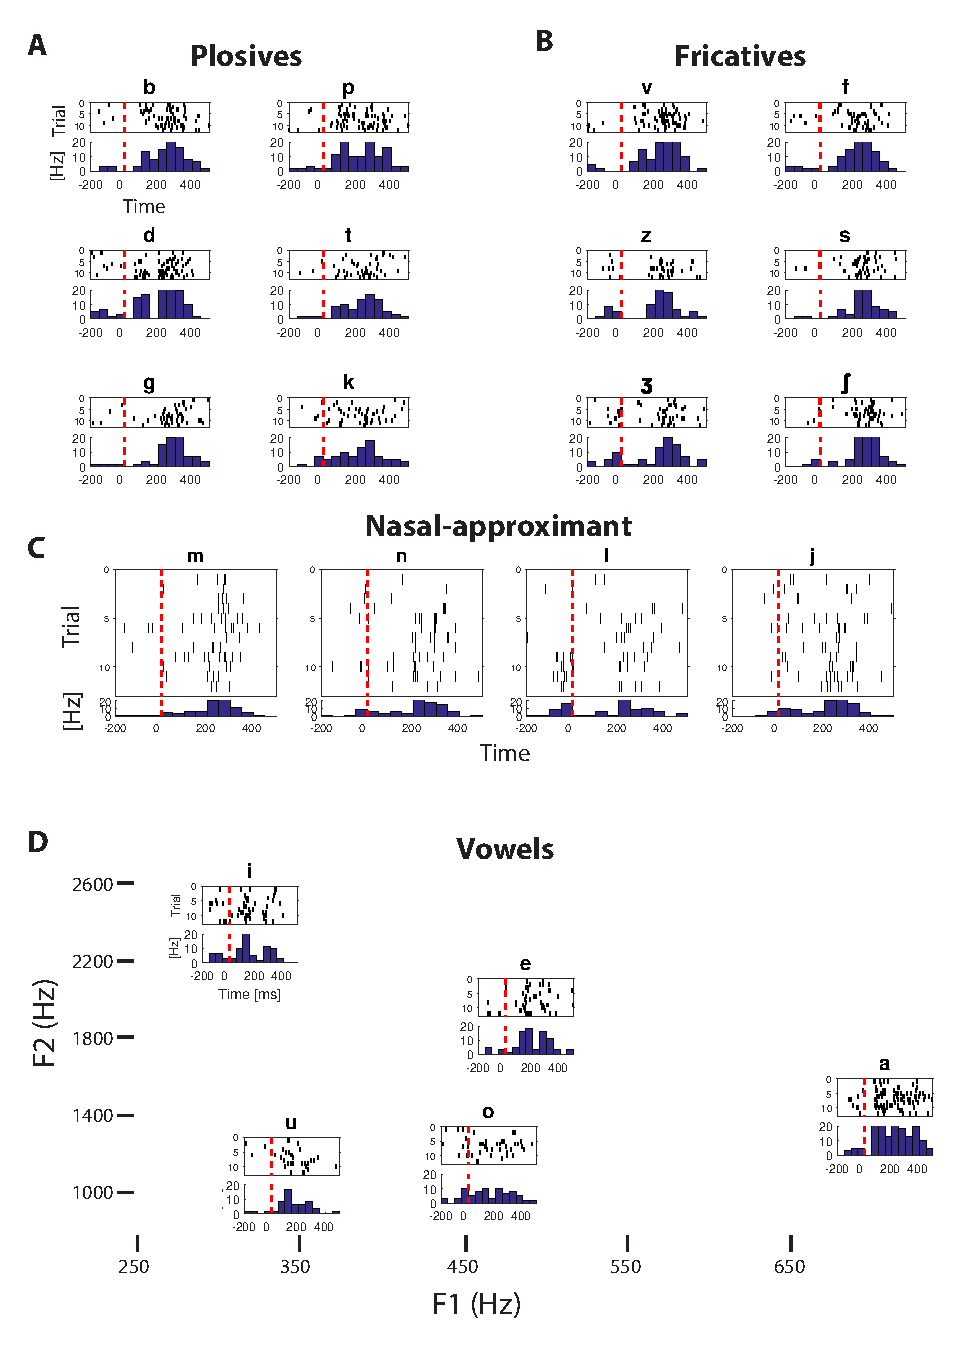
\includegraphics[width=\linewidth]{Figures/Ch3/Figure2_new.eps}
\caption{Raster and PSTH plots for an example unit, from one of the patients. (A) Voiced (left) and unvoiced (right) plosives (B) voiced (left) and unvoiced (right) fricatives (C)  nasal-approximant (left) and affricate (right) phoneme (D) Vowel rasters are embedded in approximant locations in the formant space}
\end{figure}

We describe the average responses of the fourteen selected units to all phonemes in the experiment. For each phoneme, we plot the mean firing rate in an optimal integration window (section 2.4), for which phoneme separability is maximal. Figure 2 presents mean spike-count activity in the optimal time window, for all units.

\begin{figure}[H]
\vspace{.3in}
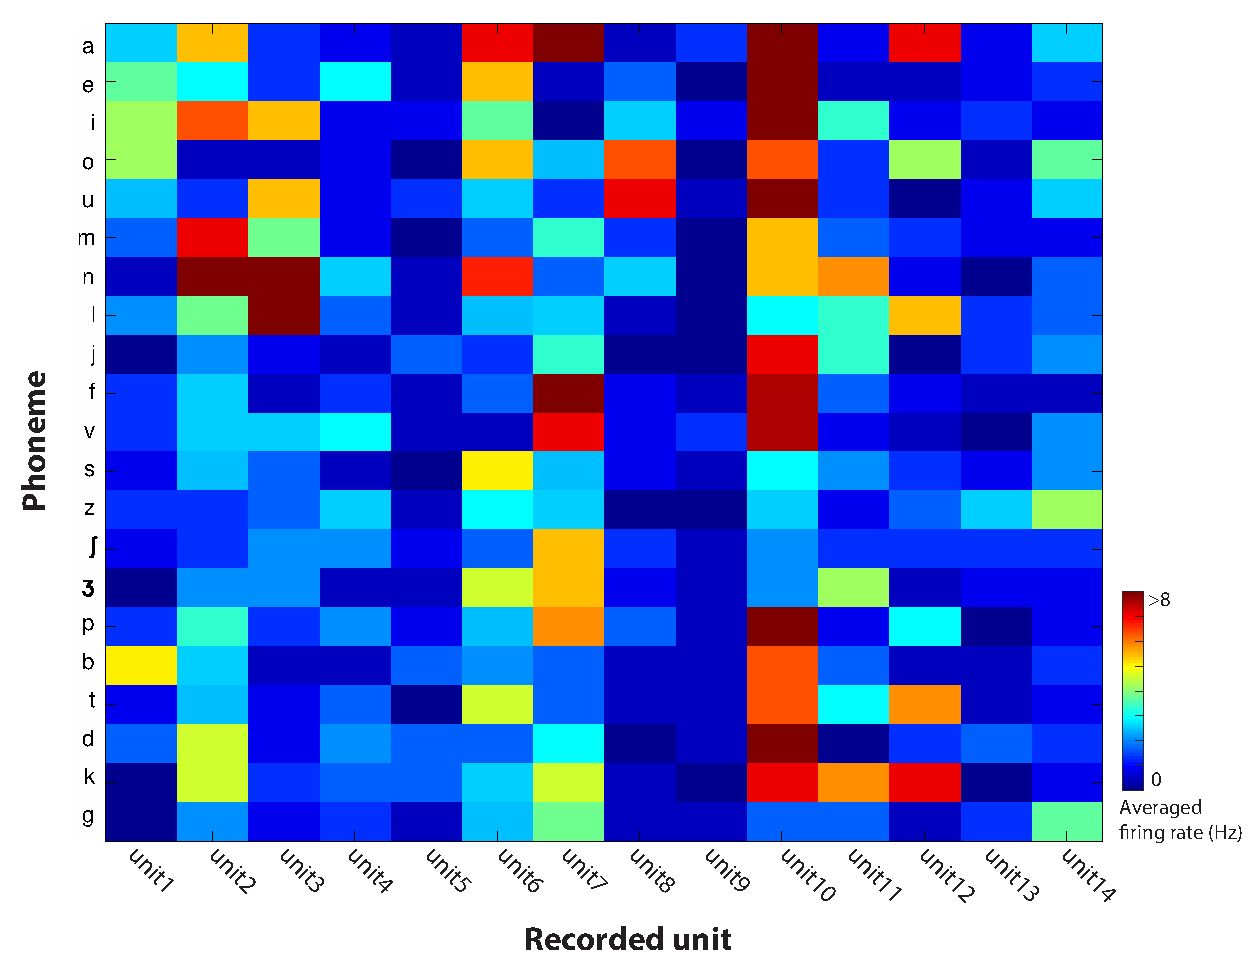
\includegraphics[width=\linewidth]{Figures/Ch3/Figure3_new.eps}
\caption{Neural tuning to phonemes for all units. Color scale represents mean spike-count activity in the optimal time window.}
\end{figure}

\subsection{The functional organization of phonemes}
Figure 2 shows that units are mainly selective to subsets of phonemes, and not to specific ones, suggesting that neural representations of phonemes are high-dimensional and distributed, yet, possibly clustered. We therefore further explore the organization of phonemes in activity space. We represent each phoneme in a high-dimensional space, in which dimensions represent mean firing rates in the time bins. Since there are fourteen units and four time bins for each, the resulting space is 48-dimensional. Next, we visualize the neural representations by projecting them into a lower-dimensional space, spanned by the three principal components of the data. Figure 3A presents the result. Sonorant phonemes - vowels (/aeiou/) and nasal-approximants(/nmlj/) - are colored in green, obstruents in blue.

\begin{figure}[H]
\vspace{.3in}
\includegraphics[width=\linewidth]{Figures/Ch3/Figure4_new.eps}
\caption{(A) Neural representations of phonemes along the first three principal components of the data. Colors: sonorant phonemes (green), obstruent phonemes (blue); (B) Hierarchical clustering. Top panel depicts a similarity matrix among the neural representations (to enhance color contrasts, diagonal values were manually set to zero). Colors: sonorant phonemes (red), obstruent phonemes (black). Bottom panel depicts hierarchical clustering of neural representations of phonemes based on single-cells recordings in the STG during listening. (C) Confusion among place-of-articulation features of consonants: labial, alveolar, palatal, velar, glottal (chance level - 0.25) (D) confusion matrix among manner-of-articulation features of consonants: plosives, fricatives, nasals, approximants and vowels.}
\end{figure}

Figure 3A suggests that sonorant and obstruent phonemes have relatively distinct neural representations. We therefore further experiment with the data in the following way. First, using hierarchical clustering, we test whether additional phonologically defined clusters of phonemes can be identified in activation space. Clusters may indicate about invariances in the neural response to specific groups of phonemes. Figure 3B presents the hierarchical clustering of the single-unit responses. A central cluster of obstruents (except for /k/, and including /e/) is observed, separated from most sonorants - the vowels /aoiu/ and nasal-approximants /nmlj/. In addition, the obstruent cluster is further divided into a sub-cluster containing all stridents /s\textipa{S}z\textipa{Z}/. 

\begin{figure}[H]
\vspace{.3in}
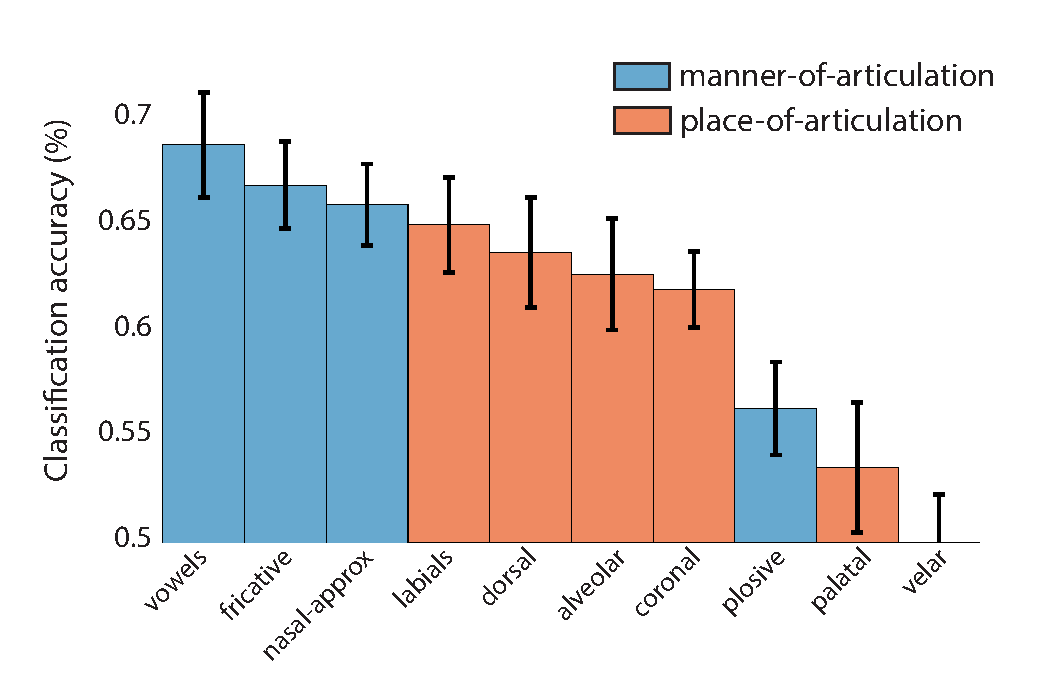
\includegraphics[width=\linewidth]{Figures/Ch3/Figure5_new.eps}
\caption{Phoneme-classification accuracy for each binary feature, e.g., [+nasals] vs. [-nasal], [+labial] vs. [-labial].}
\end{figure}

Figure 3B points to a functional organization based on manner-of-articulation features, with distinct clusters for obstruents and sonorants, and clustering of strident phonemes. However, the picture is less pronounced compared to ECoG studies. We therefore quantify and compare the invariance to manner- and place-of-articulation features directly, using probabilistic modelling. We model the spiking-pattern response to phonological features using a Naive-Bayes classifier, assuming the spike generation follows a Poisson process (section 2.5). To test invariance to features, we train the model to classify among phonemes grouped according to either manner- or place-of-articulation features. Higher classification performance indicates about higher invariance of the neural response, and classification errors indicate about similarity among phonological features. For both manner- and place-of-articulation, we label the phonemes according to four phonological features. For manner, we label /aeiou/ as 'vowel', /nmlj/ as 'nasal-approximant', /fvszS/ as 'fricative', /bdgptk/ as 'plosives'; and for place-of-articulation, /bpfvm/ as 'labial', /tdszn/ as 'alveolar', /\textipa{S}\textipa{Z}/ as palatal and /kg/ as velar. We train the classifier on a subset of the data and test predictions on a left-out data. Figure 3 (Panels C and D) presents the mean posterior distribution for all phonological features, organized in a confusion matrix - color scale indicates probability values. Only values that are significantly ($p-value<0.05$) greater than chance level are presented.

Finally, we further experiment with the data by comparing binary classification across various phonological features. For each phonological feature, e.g. [nasal], we label all phonemes as either [+nasal] or [-nasal]. We then calculate prediction accuracy based on all test trials, by taking the mode of the posterior distribution as the prediction of the model (section 2.5). Figure 4 presents prediction accuracies for various phonological features. Results are ordered from the highest to the lowest accuracy, highlighting the dominance of manner features.


\subsection{A comparison between neural and behavioral data}
Phoneme similarity in the cognitive system can be estimated from behavioral tasks, assuming the more confusable two phonemes are the more similar they are. We test whether phoneme similarity, as estimated from behavioral tasks, is reflected in the neural activity in the STG. For this, we generate two phoneme-similarity matrices - a behavioral and a neural matrix (section 2.6), and calculated the Spearman correlation between the two. We find a moderate correlation between the behavioral and neural similarity matrices ($\rho = 0.45, p-value < 10^{-3}$).


\section{Summary and Discussion}
We recorded neural activity from six patients during a listening task in which vowels and consonant-vowel syllables were aurally presented. We characterized spiking activity from fourteen neurons in the STG that were consistently responsive to the speech stimuli. We inquired into two theoretical questions. The first focused on the functional organization of phonemes in the STG. We tested whether the organization of neural representations of phonemes at the cellular level is dominated by manner-of-articulation features, as was found by previous electroencephalography studies. The second question addressed the relation between cognitive and neural representations of phoneme similarities. Using the same of stimuli as with clinical patients, we derived cognitive phoneme similarities from phoneme-confusability data in healthy subjects. We then compared the perceptual similarities to the similarities derived from population spiking activity in the STG.

To characterize single-cell responses, we calculated spike counts in an optimal time window, which is most informative about phoneme identity (Figure A.1). The optimal time window was calculated for each unit separately, as electrode locations in the STG varied between patients. Results suggest that single cells in the STG present a distributed response to phonemes, in which acoustic parameters of speech are encoded in a multi-dimensonal feature space (Figure 2). Units selective to single phonemes were not found. 

To characterize the distributed, yet possibly clustered, response patterns to different phonemes, we explored the recorded spiking activity with several methods. We first represented each phoneme in activity space in which dimensions correspond to spike counts, calculated in the most informative time window found for each unit. We then visualized the structure of phoneme representations by projecting it into a lower dimensional space (Figures 3A). The resulting structure reveals a separate representation of sonorant and obstruent phonemes, as was previously shown at the population level. The sonorant-obstruent distinction can be naturally described by acoustic correlates, but much less with gestural ones, as sonorant and obstruent phonemes have highly varied articulations.   

To further specify relations among phoneme representations, we next examined the hierarchical clustering of the data in activation space. We found that most of the sonorant and obstruent phonemes cluster separately, and that strident fricatives form a sub-cluster of the obstruent one. These results point to a functional organization, which is based on acoustic cues. Sonorants are highly resonant and have identifiable formant structure compared to obstruents. Similarly, stridents have a clear acoustic footprint, characterized by high intensity and high-frequency energy. These results are in accordance with previous ECoG studies, and point to a functional organization that is dominated by manner-of-articulation features. To further quantify this, we next trained a probabilistic classifier, which mimics the generation process of spikes, as recorded by the units. We then compared model predictions when grouping phonemes according to various phonological features. We found that model performance are significantly better when phonemes are grouped according to manner-of-articulation features, compared to place-of-articulation ones (Figures 3C-D \& 4). These results add to the accumulating evidence that neural representations in the STG are dominated by manner-of-articulation.

Finally, we compared the neural and cognitive organizations of phonemes, as estimated from single-cells activity and behavioral data, respectively. Remarkably, spiking activity from the handful of neurons reflects phoneme similarities derived from behavioral results, based on phoneme-confusion experiments using the same set of stimuli. Specifically, the nasal and approximant features show a distinct neural representation with respect to other feature classes, which corresponds to their relatively high perceptual saliency (cite).

Speech signals are composed of continuous streams of high-dimensional acoustic information, which must be encoded in the auditory pathway in a way that ensures robust categorization. The auditory pathway shows an increasing encoding specificity and invariance for speech sounds, from relatively simple acoustic features in early stages, to complex spectrotemporal acoustic patterns in cortical regions. In humans, invariance to phonetic features is thought to be found outside the primary auditory cortex, in STG and STS subregions \citep{Dewitt2012} (in animals, \citealp[see]{mesgarani2008phoneme}). This study provides another layer of evidence, showing that the functional organization of phonemes in the STG, as revealed by population spiking activity, is in accordance to auditory theories and in contrast to gestural theories of speech perception \citep{liberman1985motor, browman1992articulatory}.
